\documentclass[11pt,a4paper]{article}
\usepackage{float}
\usepackage{verbatim}
\usepackage{subfig}
\usepackage[T1]{fontenc}
\usepackage[utf8]{inputenc}
\usepackage{geometry}
\usepackage{enumitem}
%\geometry{verbose,lmargin=2cm,rmargin=2cm, bmargin=2cm, tmargin=2cm}
\usepackage{wrapfig}
\usepackage{tikz}
\usetikzlibrary{decorations.markings}
\usepackage{calc}
\usepackage{wrapfig}
\usepackage{graphicx}
\usepackage{amssymb}
\usepackage{amsmath}
\usepackage{esint}
\usepackage{hyperref}
\usepackage{listings}
\lstset{ %
  backgroundcolor=\color{white},   % choose the background color; you must add \usepackage{color} or \usepackage{xcolor}; should come as last argument
  basicstyle=\footnotesize,        % the size of the fonts that are used for the code
  breakatwhitespace=false,         % sets if automatic breaks should only happen at whitespace
  breaklines=true,                 % sets automatic line breaking
  captionpos=t,                    % sets the caption-position to bottom
  commentstyle=\color{teal},    % comment style
  deletekeywords={...},            % if you want to delete keywords from the given language
  escapeinside={\%*}{*)},          % if you want to add LaTeX within your code
  extendedchars=true,              % lets you use non-ASCII characters; for 8-bits encodings only, does not work with UTF-8
  frame=single,                    % adds a frame around the code
  keepspaces=true,                 % keeps spaces in text, useful for keeping indentation of code (possibly needs columns=flexible)
  keywordstyle=\color{blue},       % keyword style
 % language=Python,                 % the language of the code
  morekeywords={*,...},           % if you want to add more keywords to the set
  numbers=left,                    % where to put the line-numbers; possible values are (none, left, right)
  numbersep=5pt,                   % how far the line-numbers are from the code
  numberstyle=\tiny\color{black}, % the style that is used for the line-numbers
  rulecolor=\color{black},         % if not set, the frame-color may be changed on line-breaks within not-black text (e.g. comments (green here))
  showspaces=false,                % show spaces everywhere adding particular underscores; it overrides 'showstringspaces'
  showstringspaces=false,          % underline spaces within strings only
  showtabs=false,                  % show tabs within strings adding particular underscores
  stepnumber=1,                    % the step between two line-numbers. If it's 1, each line will be numbered
  tabsize=2,                       % sets default tabsize to 2 spaces
  title=\lstname                   % show the filename of files included with \lstinputlisting; also try caption instead of title
}

\begin{document}

%\preprint{APS/123-QED}

\title{FYS2150 Lab Report\\Length, Velocity and Acceleration}% Force line breaks with \\

\author{Nicholas Karlsen}
% \email{nichoka@student.matnat.uio.no}

\date{\today}% It is always \today, today,
             %  but any date may be explicitly specified

\maketitle

%\tableofcontents
\begin{abstract}
  A study on different methods for determining the length, velocity and acceleration of different objects and the errors involved in making these measurements.
\end{abstract}
\section{\label{sec:intro}Introduction}
  In this report, i will present some experimental procedures for determining the length, velocity and acceleration of three different objects; 
  \begin{itemize}
    \item Two similar, but not equal rods.
    \item A model car made of Lego
    \item An RC-car
  \end{itemize}
  Respectively. Afterward i will present my findings in performing said experiments and my interpretation of the results, and the errors involved affect these results.

\section{\label{sec:theory}Theory}
  \subsection{Pendulum}
    \begin{equation}
      \label{eqn:period}
        T \approx 2\pi \sqrt{\frac{L}{g}}\enspace
    \end{equation}
    Where $T$ denotes the period of a pendulum, $L$ its length and $g$ the gravitational acceleration. The small angle approximation (Eqn. \ref{eqn:period})  is valid for angles $\theta \ll 1\, \textup{rad}$ with an error $\approx \pm 15 \, \textup{s}$ per day \cite{pend_wik}.

  \subsection{Doppler shift}
    \begin{equation}
      f_m = f + \Delta f = \frac{c}{c-v}f  
      \label{eqn:doppler}
    \end{equation}
    Where $f_m$ denotes a measured frequency from an observer at rest, $f$ the frequency in the rest frame of a body moving relative to an observer, $\Delta f$ the Doppler shift, $c$ the speed of sound in air and $v$ the velocity of the body relative to the observer.

  \subsection{Linear Motion}
    \begin{equation}
      s = ut + \frac{1}{2}at^2
      \label{eqn:linmotion}
    \end{equation}
    Where $s$ denotes the displacement, $u$ the initial velocity, $a$ acceleration and $t$ the time. This equation is only valid when $a$ is a constant.

  \subsection{Errors}
    \begin{equation}
    \label{eqn:sigma}
      \sigma \approx \left(
      \frac{\sum x_i^2 - \frac{1}{n}(\sum x_i)^2}
      {n - 1}
      \right)^\frac{1}{2}
    \end{equation}
    
    \begin{equation}
      \label{eqn:sigma_m}
      \sigma_m \approx \left(
      \frac{\sum x_i^2 - \frac{1}{n}(\sum x_i)^2}
      {n(n - 1)}
      \right)^\frac{1}{2}
    \end{equation}

    Where $\sigma, \sigma_m$ denotes the standard deviation, and the standard deviation of the mean respectively of a set of $n$ values $x_i$. \cite{squires}.

    Any errors stated in a derived number will be calculated using the equations for combinations of errors found on page 29 in Squires \cite{squires}. Lastly, when using a linear fit on a set of linearly correlated data i used the expressions found on page 39 in Squires \cite{squires} to calculate the regression line, as well as its error.

\section{\label{sec:exp_proced}Experimental Procedure}
 
  \subsection{Measuring the difference in lengths between two rods}
    \subsubsection{Measurements using the Hultafors meter ruler}
      The rod was placed on a flat surface, and the end of the rod was lined up with the $1cm$ marker on the Hultafors Meter ruler in order to negate any effect the "wear and tear" of the ruler might have on the results. This $1cm$ difference was accounted for in our reading of the data. The ruler was laid down on the table along with the rod, and did flex slightly because of this. The error due to flex is accounted for in the error section of the data sheet provided by the manufacturer. This procedure was repeated for both rods a and b.

    \subsubsection{Measurements using the Bosch PLR30}
      The rods were placed and secured to the table using adhesive tape on a table whilst being in direct contact with a wall. The Bosch PLR30 Laser range finder \cite{PLR}, henceforth referred to as "laser", was then placed at the opposing end of the rod in order to measure the length from there, to the wall. Since the rod was touching the wall, this effectively means that we measured the length of the rod. There was a slight degree of systematic error in our procedure, as we could not ensure that the laser was pointing with exact parallel to the rod, nor did we have an exact way of placing the laser such that its origin would be at the exact end-point of the rod. 

    \subsection{Measurement using a digital vernier caliper}
      In order to determine the difference in length between the two rods directly we used a digital vernier caliper \cite{cocraft}. The rods were secured to a table in parallel, right next to each other with the ends on one side lined up with each other. The measurement of the difference in their lengths was then made on the other side using the vernier caliper. The vernier caliper was held above the two rods, resting on them in order to minimize any systematic error.

  \subsection{Measuring the period and height of the Foucault's pendulum}

    \subsubsection{\label{subsect:exp_period}Measuring the period of the pendulum}
    The measurements were taken in sequence using the lap function of the Cielo 100MT \cite{cielo} stopwatch. The time was recorded every other apex of the swing, which amounts to one period. All of the measurements were taken by the same person in order to ensure that the error in judgment and reaction time would remain the same throughout all of the measurements.

    \subsubsection{Measuring the height of the center of mass}
      In order to perform this measurement two people stood on opposing sides of the enclosure, as shown in Fig \ref{fig:pendelfy}. One rested a meter ruler up against the glass enclosure and standing on the floor, whilst the other pointed a laser from the other side. The laser was pointed to the meter ruler whilst held horizontally. Then, while the pendulum was still in motion, the laser was progressively adjusted during each swing until it was just below the lowest point of the pendulums trajectory, repeated this to if. Needless to say, this is a highly inaccurate measurement, and there is no precise way to determine the magnitude of the error in this reading as it is almost entirely due to a systematic fault in our method.
      \begin{figure}[H]
        \center 
        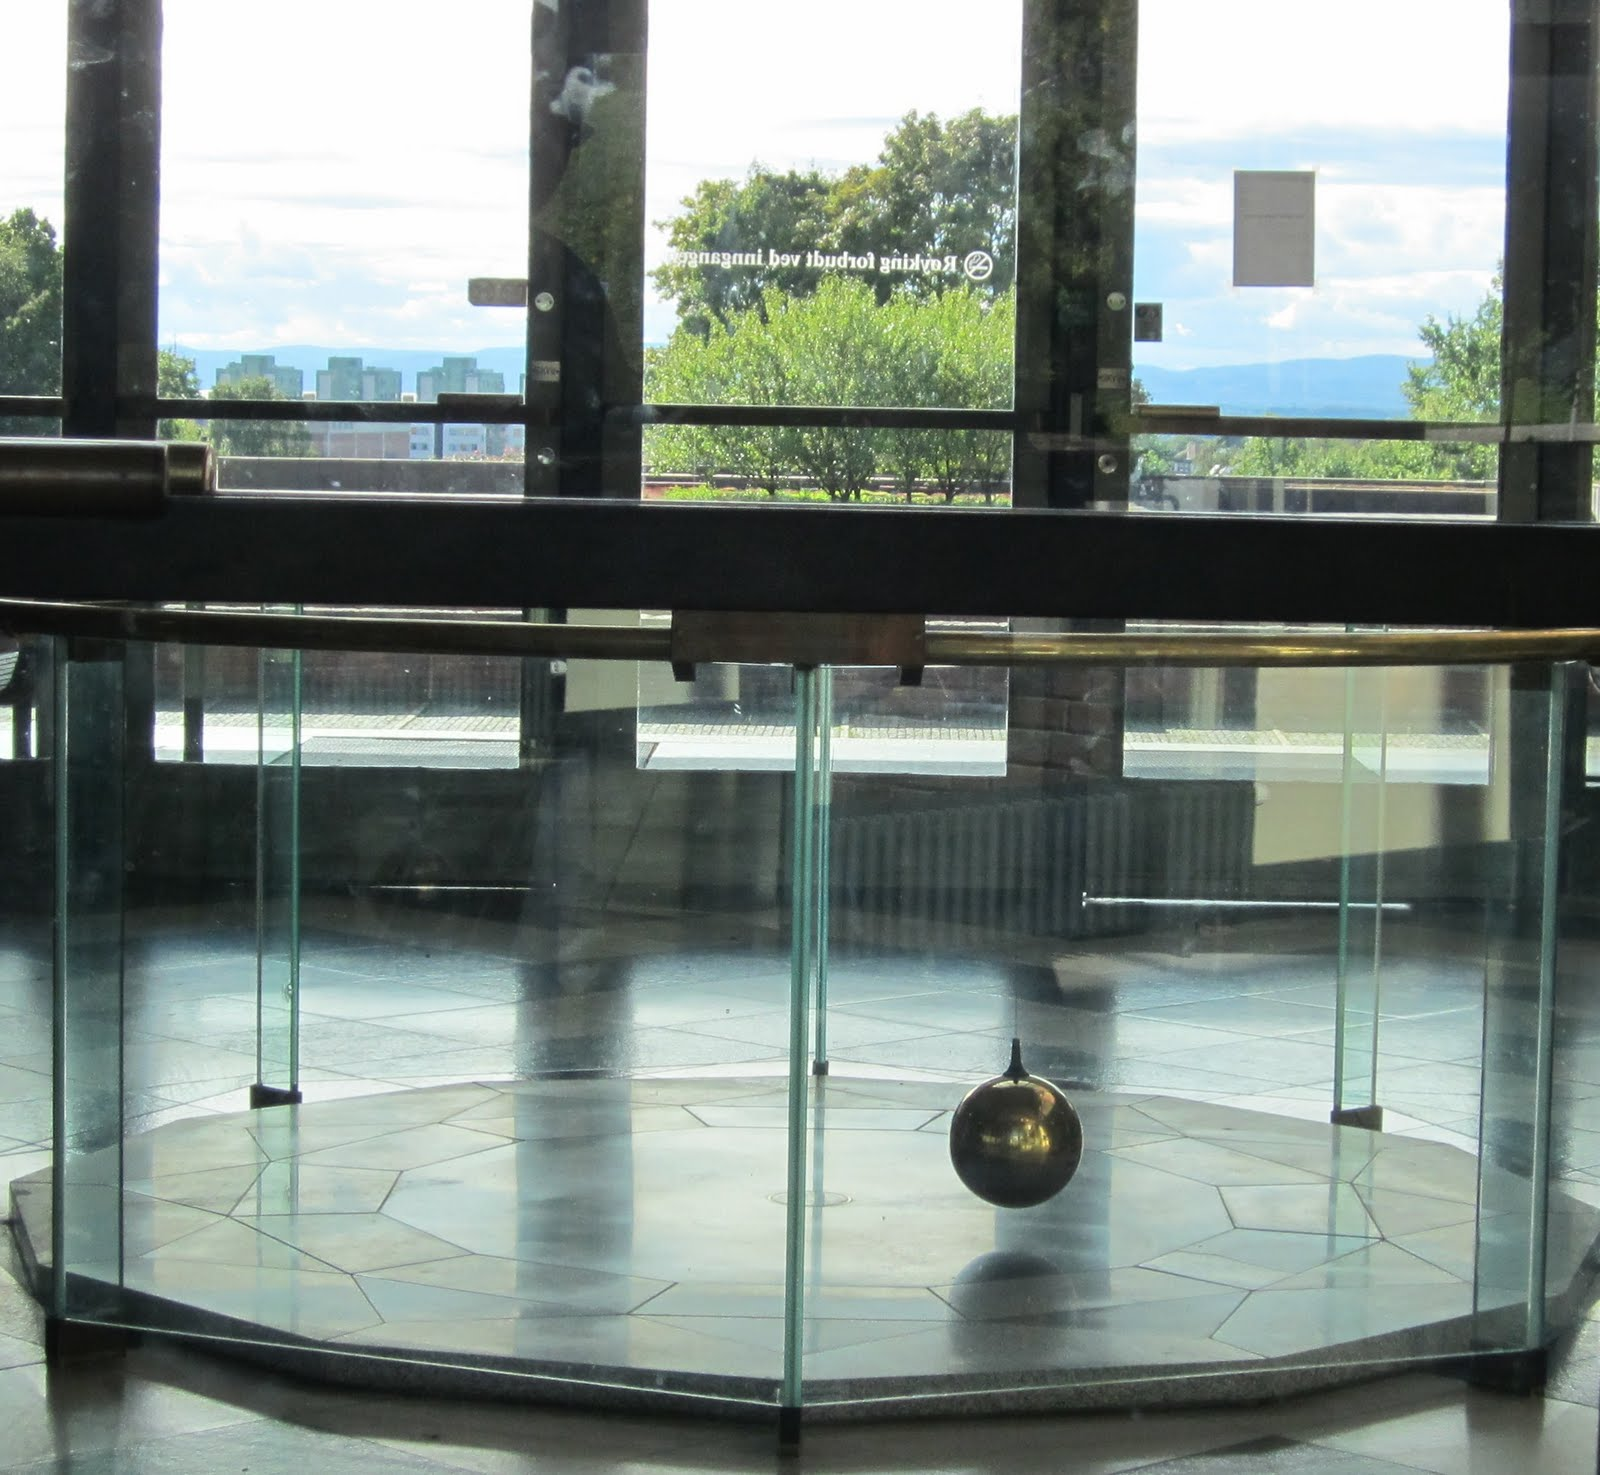
\includegraphics[scale=0.15]{scripts/figs/pendelimg.JPG}
        \caption{A photograph of the Foucault's Pendulum at UiO.}
        \label{fig:pendelfy}
      \end{figure}

    \subsubsection{Measuring the height of the roof}
      The Laser rangefinder \cite{PLR} was placed on the floor of the entrance hall, turned on and the measured value was recorded in the lab journal.


  \subsection{Measuring the acceleration of a lego-car}
    A model car made of Lego, with an attached speaker emitting a sound with constant frequency was placed on a ramp with variable height and constant length as sketched in Fig. \ref{fig:rampsketch}.
    \begin{figure}[H]
      \center
      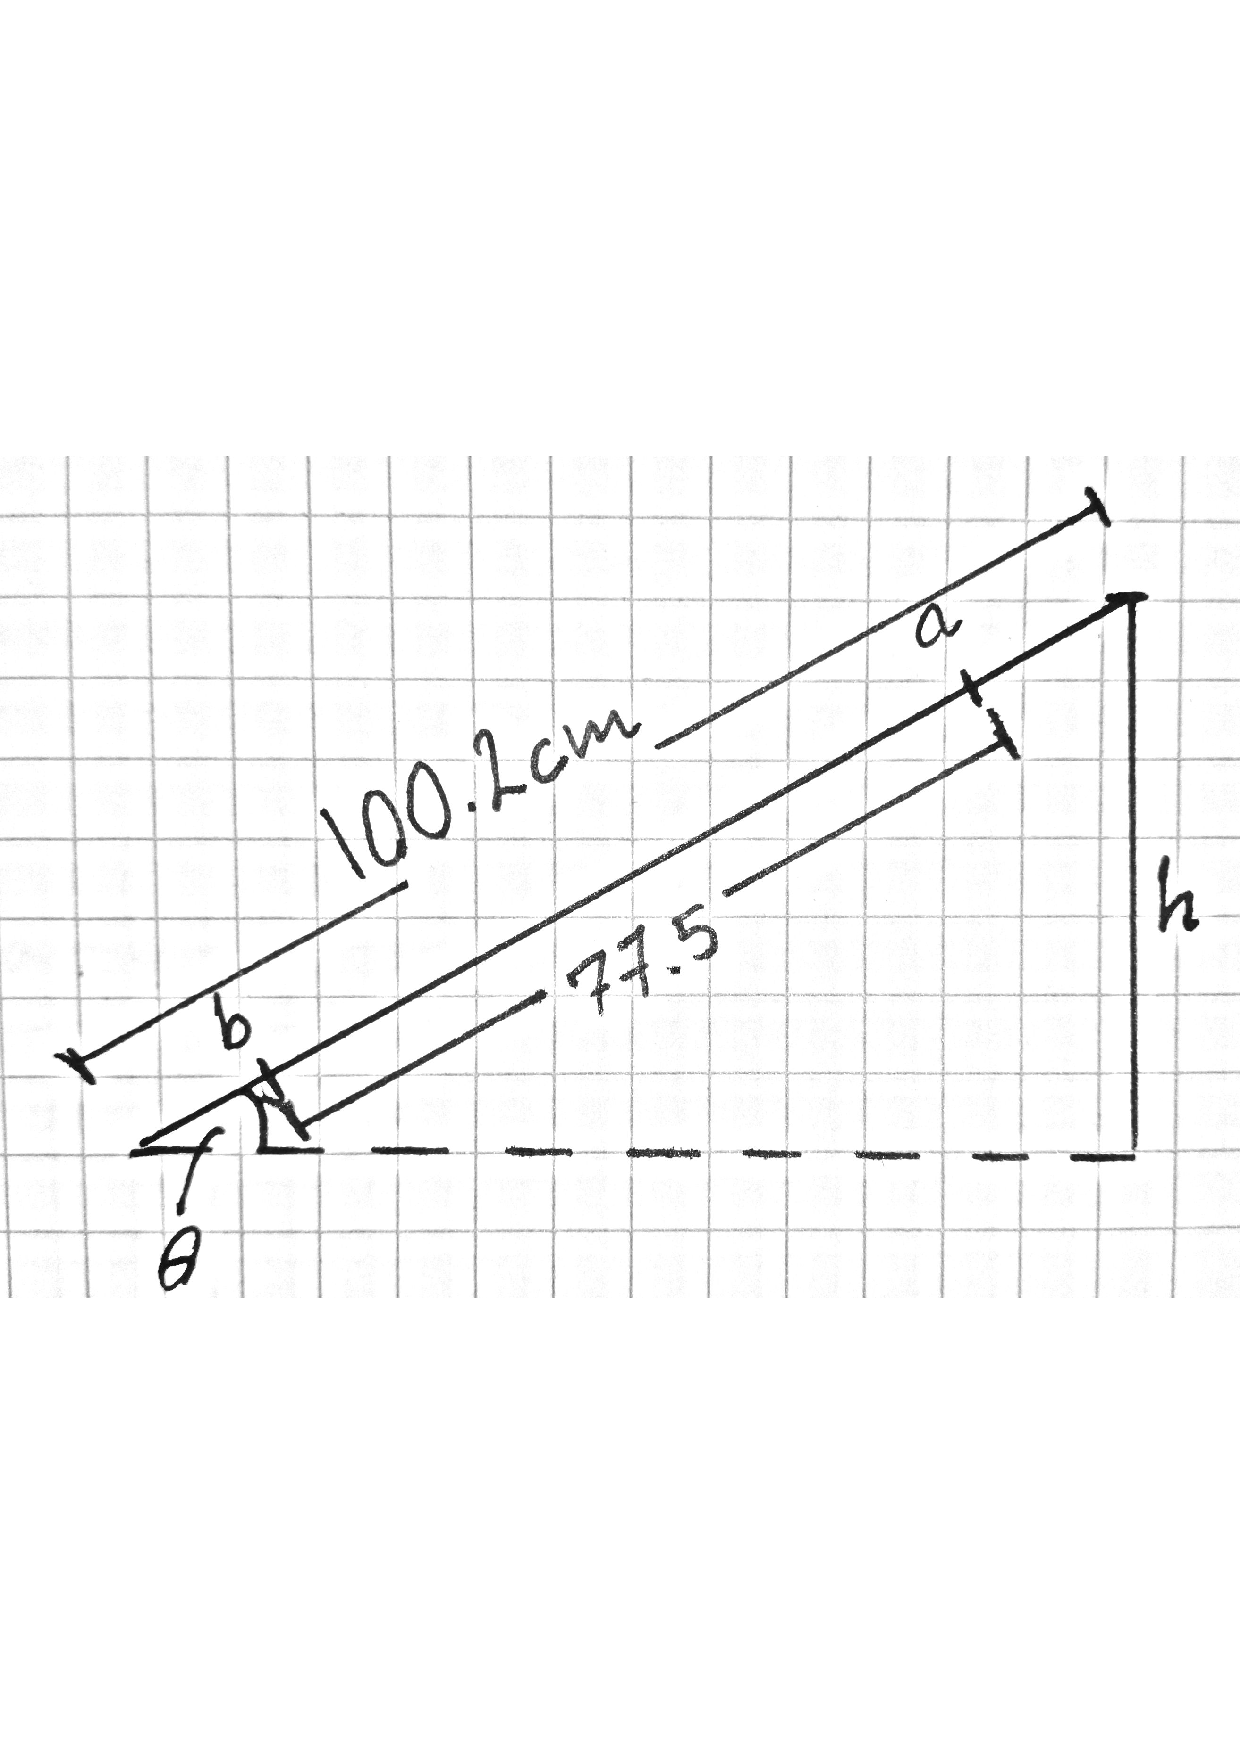
\includegraphics[scale=0.3]{scripts/figs/legodiag.pdf}
      \caption{Sketch showing the properties of the ramp used}
      \label{fig:rampsketch}
    \end{figure}
    The model car was released with its nose at point a (marked with black adhesive tape) and accelerated by gravity until its nose hit point b (also marked with black adhesive tape). This was timed using a stopwatch by the same person who made the measurements in section \ref{subsect:exp_period}. At the bottom of the ramp there was a microphone connected to a PC with matlab which collected sound data. Several people conducted similar experiments in the same room and at the same time, so the microphone may have picked up other signals as well.

    The experiment was repeated 3 times, with varying heights, $h$.
  
  \subsection{Measuring the velocity of the RC-car}
    An RC-Car with an attached speaker emitting a sound with constant frequency was driven along the floor. The sound was recorded with a microphone connected to a PC running matlab. The car was driven on a linoleum floor, so its wheels did not grip as well as one might hope. It was also not driven perfectly straight, so the maximum velocity of the car may not have been reached. There was also not much room for the car to reach this velocity either.


\section{\label{sec:data} Results}

  \subsection{Rod measurements}
    \begin{table}[H]
      \center
      \caption{Length of rods}
      \label{tab:lenrods}
      \begin{tabular}{rrrrrrrrr}
\hline
Ruler & Ruler & Ruler & Ruler & Laser & Laser & Laser & Laser & Vernier Calliper \\
   $l_a [cm]$ &  $\delta l_a$ [cm] &   $l_b$ [cm] &   $\delta l_b$ [cm] &   $l_a$ [cm] &   $\delta l_a$ [cm] & $l_b$ [cm] &   $\delta l_b$ [cm] & $l_{a, b}$ [mm] \\
\hline
           119.50 &              0.23 &           119.60 &              0.23 &           120.50 &              0.20 &           120.60 &              0.20 &                         1.25 $\pm 0.05$ \\
           119.50 &              - &           119.70 &              - &           119.60 &              0.20 &           119.80 &              0.20 &                         - \\
           119.45 &              0.37 &           119.60 &              0.37 &           119.50 &              0.20 &           119.70 &              0.20 &                         1.40 $\pm 0.05$\\
           119.40 &              - &           119.50 &              - &           119.40 &              0.20 &           119.60 &              0.20 &                         - \\
           119.43 &              0.40 &           119.55 &              0.40 &           119.40 &              0.20 &           119.60 &              0.20 &                         1.20 $\pm $0.6\\
           119.40 &              0.20 &           119.60 &              0.20 &           119.68 &              0.20 &           119.72 &              0.20 &                         1.80 $\pm $0.05\\
           119.40 &              0.27 &           119.50 &              0.27 &           119.90 &              0.20 &           119.70 &              0.20 &                         0.00 $\pm 0.05$\\
           119.45 &              0.35 &           119.65 &              0.35 &           130.60 &              0.20 &           130.20 &              0.20 &                         1.80 $\pm $0.05\\
           119.40 &              - &           119.60 &              - &           119.40 &              0.22 &           119.50 &              0.22 &                         - \\
           119.43 &              0.31 &           119.55 &              0.31 &             - &              - &             - &              - &                         1.50 $\pm 0.05$\\
\hline
\end{tabular}

    \end{table}
    Table. \ref{tab:lenrods} contains all the measurements made of the rods by the Tuesday group, copied from the \href{https://uio.instructure.com/courses/910/modules/items/13592}{image} posted on canvas. Some of the data was not clearly readable, and has therefore been omitted from this table. The measurements made by me and my lab parter are located in row 1 of table \ref{tab:lenrods}.

    \begin{table}[H]
      \center
      \caption{Derived data from table \ref{tab:lenrods}}
      \begin{tabular}{| l | l | l | l | l | l | l | l | l | l |}
\hline
    -  & $\bar{l_{a}}$ & $\sigma_a$ & $\sigma_{m, a}$ & $\bar{l_{b}}$ & $\sigma_b$ & $\sigma_{m, b}$ & $\bar{l_{ab}}$ & $\sigma_{ab}$ & $\sigma_{m, ab}$ \\ \hline

    Ruler  & $\bar{l_{a}}$ & $\sigma_a$ & $\sigma_{m, a}$ & $\bar{l_{b}}$ & $\sigma_b$ & $\sigma_{m, b}$ & $\bar{l_{ab}}$ & $\sigma_{ab}$ & $\sigma_{m, ab}$ \\ \hline

    Laser  & $\bar{l_{a}}$ & $\sigma_a$ & $\sigma_{m, a}$ & $\bar{l_{b}}$ & $\sigma_b$ & $\sigma_{m, b}$ & $\bar{l_{ab}}$ & $\sigma_{ab}$ & $\sigma_{m, ab}$ \\ \hline

\end{tabular}
      \label{tab:lenrods2}
    \end{table}

    \begin{table}[H]
      \center
      \caption{Uncertainty in Length measurement using the meter ruler}
      \label{tab:uncert}
      \begin{tabular}{| l | l | l |}
\hline
 & $x$ & $\delta x$ \\
\hline
$l_a$                 & $119.5cm$ &    \\             
$l_b$                 & $119.6cm$ &    \\        
$dl_s$                &     & $1.4mm$   \\             
$\sqrt{n}\cdot dl_l$  &     & $0.5\sqrt{5}mm$   \\                  
$dl_m$                &     & $1.4mm$   \\                  
$\alpha l_a (T-25C)$  & $-0.156cm$ & $\sim 10^{-6}$   \\ 
\hline                

\end{tabular}

\begin{tabular}{| l | l | l |}
\hline
& $\sum x_i$ & $\sqrt {\sum \sigma x_i^2 }$ \\
\hline
$\sum l_a$ & 119.48cm & 2.27 \\
$\sum l_b$ & 119.58cm & 2.27 \\
\hline   
\end{tabular}
    \end{table}
    
    \begin{itemize}
      \item $l_a, \enspace l_b:$ Recorded length of rod $a$ and $b$ respectively
      \item $dl_s:$ Error due to aiming of the ruler
      \item $\sqrt n \cdot dl_l:$ Error due to curvature of joints
      \item $dl_m:$ Error due to precision of measuring lines
      \item $\alpha :\enspace 4\cdot10^{-5\circ} C^{-1}$, Coefficient of linear thermal expansion for glass fiber
    \end{itemize}

  \subsubsection{Pendulum measurements}
    \begin{table}[H]
      \center
      \caption{Period of pendulum}
      \label{tab:pendel}
      \begin{tabular}{rrrr}
\hline
   T [s]\\
\hline
    7.30\\ 7.72\\ 7.57\\ 7.43\\ 7.73\\ 7.27\\ 7.68\\ 7.60\\ 7.34\\ 7.75\\
    7.06\\ 7.32\\ 7.55\\ 7.29\\ 7.08\\ 7.82\\ 7.78\\ 7.44\\ 7.68\\ 7.46\\
\hline
\end{tabular}

    \end{table}
    \begin{figure}[H]
      \center
      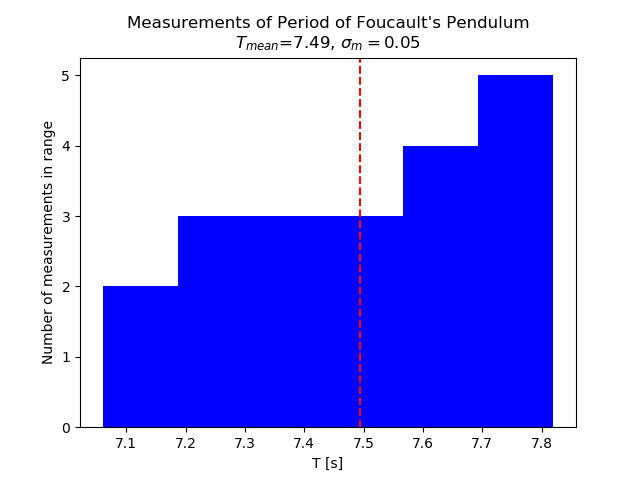
\includegraphics[scale=0.7]{scripts/figs/period.png}
      \caption{Measurements of the Period of the Foucault's Pendulum in the entrance hall at the Institute of Physics, UiO.}
      \label{fig:pendel}
    \end{figure}

    \begin{align}
      \begin{split}
        h_{F, t} &= 28cm \\
        h_{F, b} &= 8cm \\
        \label{eqn:pend_height}
      \end{split}
    \end{align}

    Where $h_{F, t}, h_{F, b}$ in Eqn. \ref{eqn:pend_height} denote the distance measured from the floor to the top and bottom of the Foucault pendulum respectively. These readings imply that the center of mass, $h_{F, cm} = 18cm \pm \delta h_{F, cm}$, where $\delta h_{F, cm}$ is a potentially large error of unknown size due to systematic faults in our procedure. More on this in the discussion.
    \newline
    \newline
    The height of the ceiling was measured using the Bosch PLR30 to be $H_C = 13.878m \pm 0.003$.
    \newline
    \newline
    From Eqn. \ref{eqn:period} i calculate the length from the fix point of the pendulum to its center of mass, denoted by L. Using the mean period $\bar T$ and its error $\delta \bar T = \sigma_m$. The error in $L$ is then found using the equations on page 29 in squires \cite{squires}.
    \begin{align}
      \begin{split}
      L &= g\frac{\bar T^2}{4\pi} \pm 2\bar T\delta \bar T\\ &= g\frac{\bar T^2}{4\pi} \pm 2\bar T\sigma_m \\&=13.94 \pm 0.75\,m
      \end{split}
    \end{align}

    This, along with $h_{F, cm}$ and the height of the roof lets me find the height of the fix point above the floor, $H_F$.

    \begin{equation}
      H_F = h_{F, cm} + L = 14.12 \pm \sqrt{\delta h_{F, cm}^2 + 0.75^2}m
    \end{equation}

    Which means that distance from the ceiling to the fix point, $d$ is 
    \begin{equation}
      d = H_F - H_C = 0.24 \pm \sqrt{\delta h_{F, cm}^2 + 0.75^2 + 0.003^2}m < 0.24 \pm 0.77m
      \label{eqn:d}
    \end{equation}

    My reasoning for the inequality stated in Eqn. \ref{eqn:d} will be elaborated in the discussion later.

  \subsubsection{Lego-car measurements}

    \begin{figure}[H]%
      \centering
      \subfloat[]{{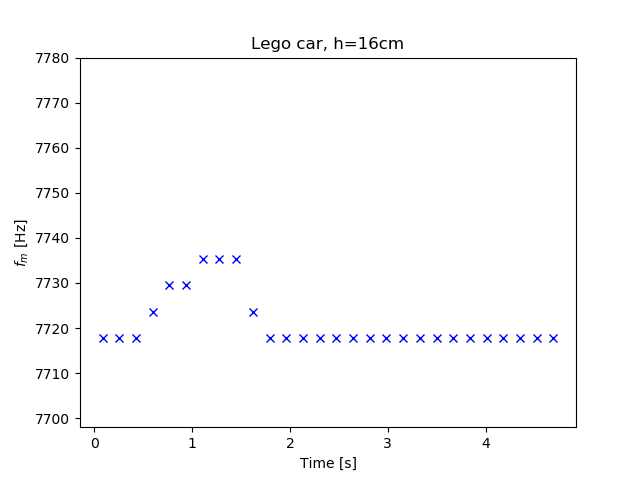
\includegraphics[width=9cm]{scripts/figs/lego16cm_freq.png}}}
      \subfloat[]{{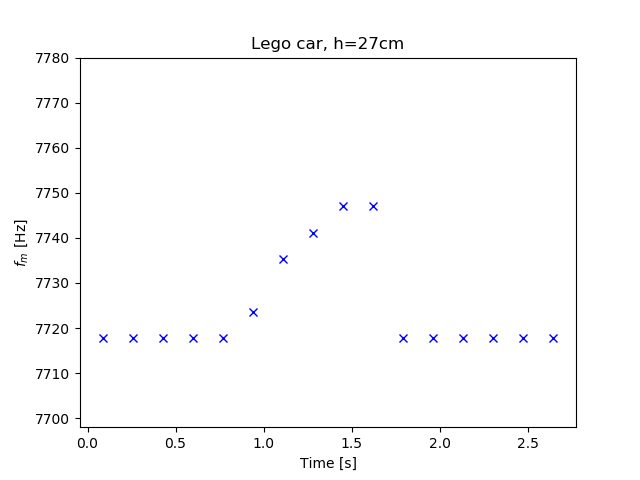
\includegraphics[width=9cm]{scripts/figs/lego27cm_freq.png}}}\\
      \subfloat[]{{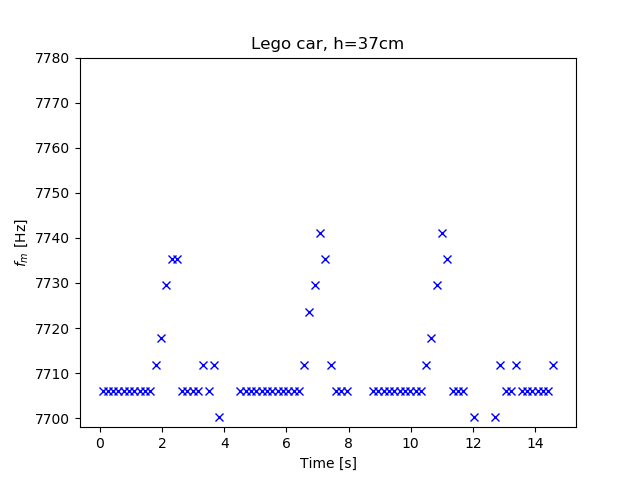
\includegraphics[width=9cm]{scripts/figs/lego37cm_freq.png}}}
      \caption{}%
      \label{fig:legocar_fre}%
    \end{figure}

    Shown in Fig \ref{fig:legocar_fre} are the measured frequencies recorded by the microphone. From this data, the frequency emitted from the speaker when at rest is $7718\, Hz$. This value is used when deriving the values shown in the following plots to calculate the relative velocity of the lego car when it is moving down the ramp using Eqn. \ref{eqn:doppler}. In this data set, the car is moving down the ramp when $\Delta f_M > 0$ and $f_m > 7718$.

    \begin{figure}[H]%
      \centering
      \subfloat[]{{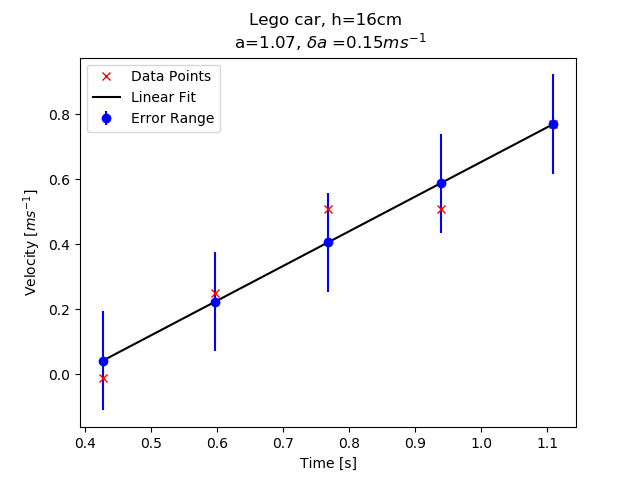
\includegraphics[width=9cm]{scripts/figs/lego16cm.png}}}
      \subfloat[]{{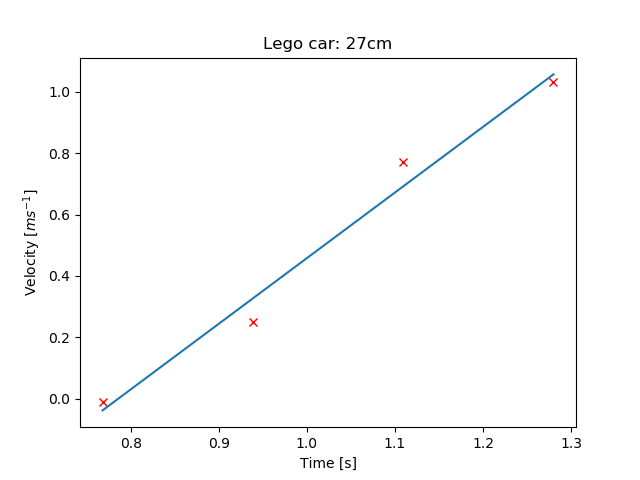
\includegraphics[width=9cm]{scripts/figs/lego27cm.png}}}\\
      \subfloat[Attempt 1]{{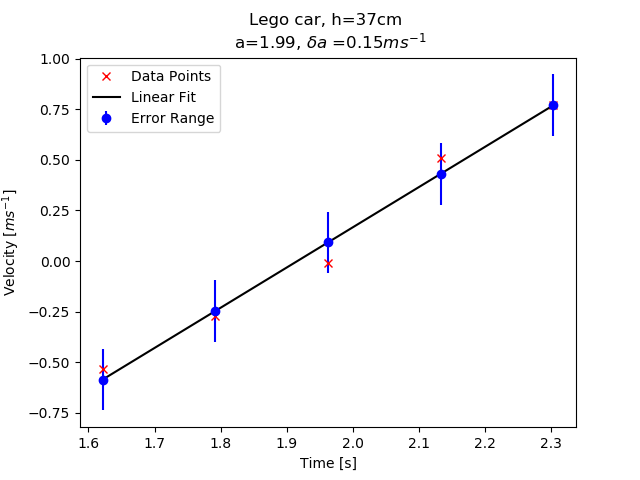
\includegraphics[width=9cm]{scripts/figs/lego37cm1.png}}}
      \subfloat[Attempt 2]{{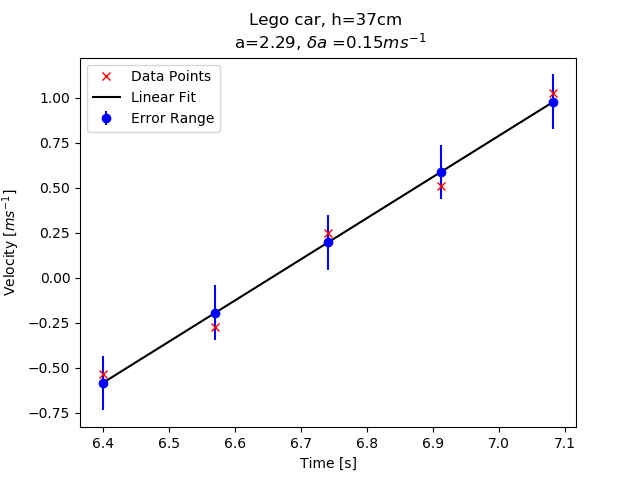
\includegraphics[width=9cm]{scripts/figs/lego37cm2.png}}}\\
      \subfloat[Attempt 3]{{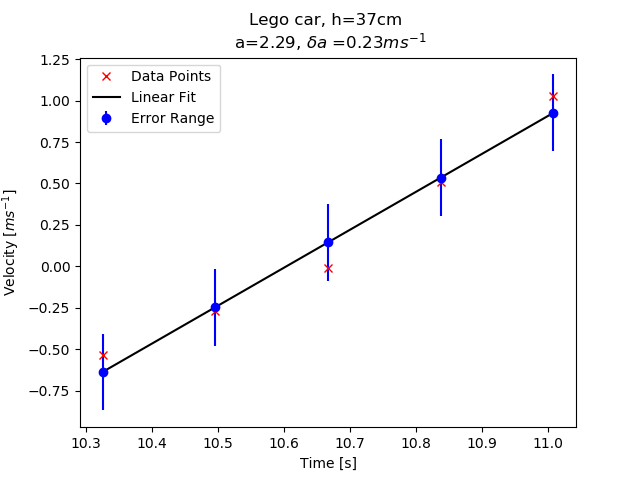
\includegraphics[width=9cm]{scripts/figs/lego37cm3.png}}}
      \caption{}%
      \label{fig:legocar}%
    \end{figure}

    Shown in Fig. \ref{fig:legocar} are the relevant, selected data points of data derived from the measured frequencies, labeled by the height of the ramp from which the car was released. Also in the title is the gradient, $a$ and the error in the gradient, $\delta a$ of the regression line. In this case, representing the acceleration of the Lego car. 
  
  \begin{table}[H]
    \center
    \caption{Time for car to travel down ramp measured using stopwatch}
    \label{tab:legocar2}
    \begin{tabular}{| l | l | l | l |}
\hline
    Height [cm]  & Time [s] & $a_{theoretical}$ $[ms^-2]$ & $\delta a_{theoretical}$\\ \hline
    16.9         & 1.2  & 0.99 &  0.44   \\ \hline
    27.2         & 0.8  & 2.42 &  1.07   \\ \hline
    37.1         & 0.82 & 2.30 &  1.01   \\ \hline
\end{tabular}
  \end{table}

  In table \ref{tab:legocar2}, the time was measured using a stopwatch, the theoretical acceleration is calculated using Eqn. \ref{eqn:linmotion} with $\delta a_{theoretical}$ calculated using the standard deviation of the measurements made of the pendulum period, $\pm0.23\,s$ error in the stopwatch measurements. As it roughly correlates to the reaction time of the person who took the measurements.



  \subsubsection{RC-car measurements}
      \subsubsection{Lego-car measurements}

    \begin{figure}[H]%
      \centering
      \subfloat[]{{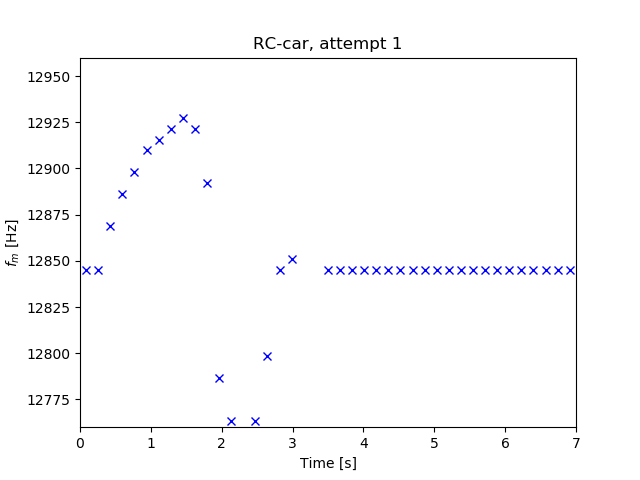
\includegraphics[width=9cm]{scripts/figs/RC_1freq.png}}}
      \subfloat[]{{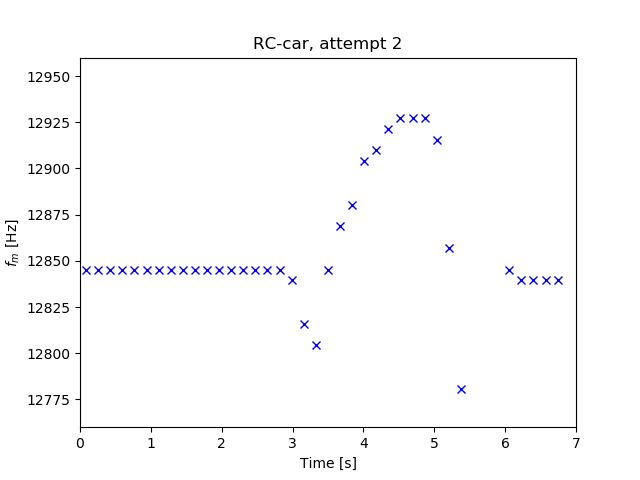
\includegraphics[width=9cm]{scripts/figs/RC_2freq.png}}} \\
      \subfloat[]{{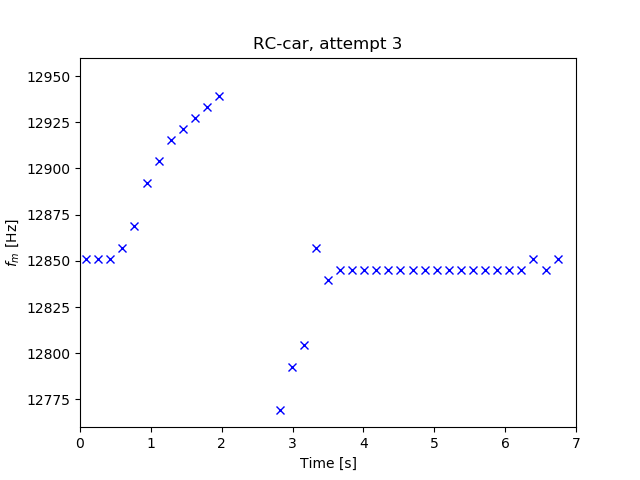
\includegraphics[width=9cm]{scripts/figs/RC_3freq.png}}}
      \caption{}%
      \label{fig:rc_freq}%
    \end{figure}

    \begin{figure}[H]%
      \centering
      \subfloat[]{{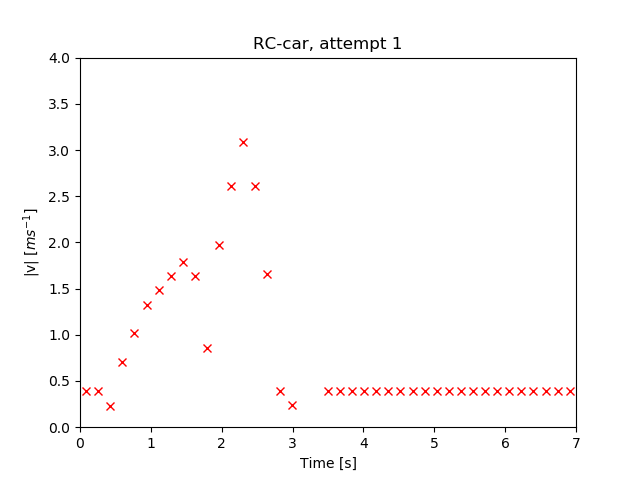
\includegraphics[width=9cm]{scripts/figs/RC_1abs.png}}}
      \subfloat[]{{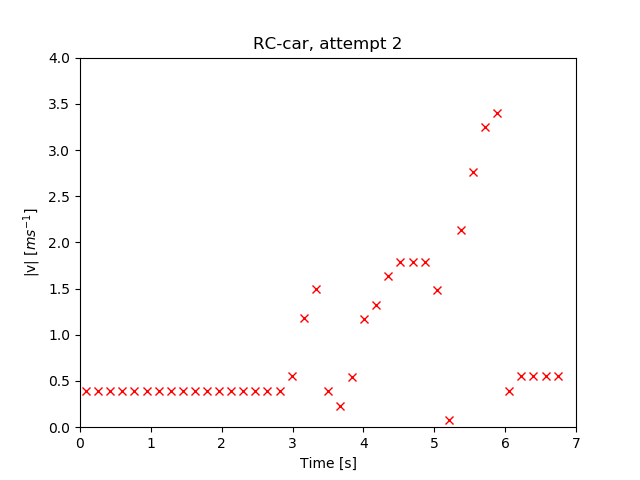
\includegraphics[width=9cm]{scripts/figs/RC_2abs.png}}} \\
      \subfloat[]{{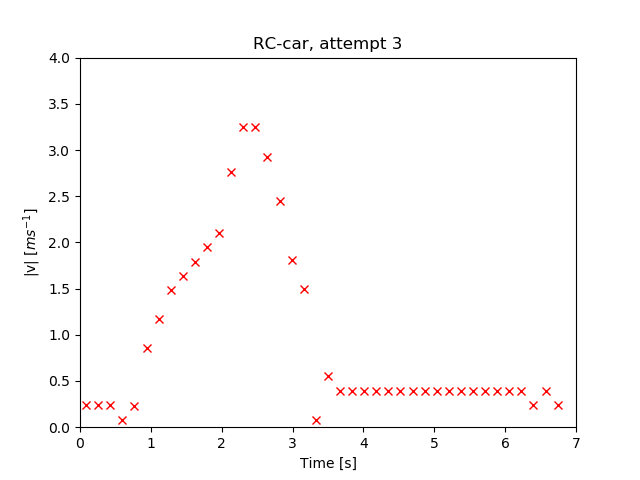
\includegraphics[width=9cm]{scripts/figs/RC_3abs.png}}}
      \caption{}%
      \label{fig:rc_exp}%
    \end{figure}

    Shown in Fig. \ref{fig:rc_exp} is the absolute value of the velocities derived from the data shown in \ref{fig:rc_freq}. More on this in the discussion.


\section{\label{sec:disc}Discussion}
  \subsection{Length of rods}
    When looking the data presented in table \ref{tab:lenrods} and its derived values in table \ref{tab:lenrods2}, the biggest outlier in what was expected is the data from the measurements made with the Laser range finder. Whilst its instrumental error is lower than with the meter rule, the spread in values, $\sigma$ and $\sigma_m$ on table \ref{tab:lenrods2} show to be much greater than for the measurements made with the ruler. This suggests that while the instrument itself is more accurate in comparison to the meter rule, the risk of systematic error is much greater than in the case of the meter rule, with its remarkably low standard deviations. What could be the cause of this? First of all, finding a reliable method of taking the measurements are not as obvious, and intuitive, as when using the meter ruler. Two readings in particular, of size $\sim 130cm$ show up in $l_a,\, l_b$ for the laser. Considering the approximate size of the PLR30 range finder is $\sim 10cm$, this suggests to me that there may have been some confusion as to where the laser measures its distance from; the top or bottom of the instrument? 

  \subsection{Pendulum}
    To address my statement in Eqn. \ref{eqn:d}, where i claim that the uncertainty in my derived value $d$ must be less than $\pm 0.77m$. To arrive at this particular value, i assumed the error $\delta h_{f, cm} = 0.18m$, a rather liberal assumption, but as it turns out, quite an irrelevant one. As it turns out, the error brought on when measuring the period, $\sigma_m$, accounts for the majority of the error in the calculated value for $d$. So any efforts in trying to minimize the error $h_{F, cm}$ would be largely wasted unless $\sigma_m$ was reduced. Therefore, since i don't have any exact, scientific method of determining $\delta h_{f, cm}$, i will simply state my final uncertainty $\delta d \approx 0.77m$. Which of course is an unacceptably large range, as it could potentially put the fix point of the pendulum below the ceiling, which i know to be false.

  \subsection{Acceleration of Lego-car}
    In this experiment, we made two measurements. The audio recording, which was used to find the acceleration of the Lego car with Eqn. \ref{eqn:doppler}, and by timing the distance it took for the car to go down the track. As seen in \ref{tab:legocar2}, the theoretical result is highly inaccurate, largely due to the short timespan on the experiment and the relatively large contribution in error from the reaction time of the person operating the stopwatch. Since our track was rather short, this data becomes essentially worthless. The data derived from the audio on the other hand, seems to be a fair bit better. The data is far more consistent and the range of uncertainty is reasonably small compared to the measured values. There were some variations in the values we got when repeating the experiment with the same parameters, but the value ranges did all overlap, so nothing to be alarmed about.

  \subsection{Velocity of the RC-car}
    Looking at the data presented in Figs. \ref{fig:rc_freq}, \ref{fig:rc_exp}, i do not believe i can make any firm decision as to what the max speed of the RC-car might be. Ideally, i would be looking for a flat line in one of $|v|/t$ graphs. But no such line seems to be present. I believe this can largely be attributed to a poorly conducted experiment. The experiment itself, was performed in a rushed manner because we had certain time constraints to deal with. We also struggled greatly to keep the RC-car going in a straight line, meaning it would spin out partway through the measurement. Ultimately, a car on a fixed track, or something similar to restrict its motion would have been proffered. There was also an issue of accelerating the car enough to actually get to top speed before having to break, due to having conducted the experiment in a rather small room.

\section{\label{sec:conc}Conclusion}
  From this, i believe i have gotten a much better insight into the many problems and considerations that goes into measuring such seemingly basic properties such as length, velocity and acceleration. How the errors manifest in these experiments, and then go on to propagate into any derived results we find using these measurements. And ultimately, the value in repeated, identical measurements when trying to measure the true value of something. 

\begin{thebibliography}{1}

\bibitem{pend_wik}
\url{https://en.wikipedia.org/wiki/Pendulum}.

\bibitem{squires}
G.~L. Squires.
\newblock {\em Practical Physics 4th Edition}.
\newblock Cambridge University Press, 2001.

\bibitem{cocraft}
\url{http://www.uio.no/studier/emner/matnat/fys/FYS2150/v18/kursmateriell/datablader-og-brukermanualer/cocraft-digitalskyvel%C3%A6r.pdf}

\bibitem{hultafors}
\url{http://www.uio.no/studier/emner/matnat/fys/FYS2150/v18/kursmateriell/datablader-og-brukermanualer/hultafors_meterstokk.pdf}

\bibitem{PLR}
\url{http://www.uio.no/studier/emner/matnat/fys/FYS2150/v18/kursmateriell/datablader-og-brukermanualer/bosch_plr30.pdf}

\bibitem{cielo}
\url{http://www.uio.no/studier/emner/matnat/fys/FYS2150/v18/kursmateriell/datablader-og-brukermanualer/stoppeklokke.pdf}

\end{thebibliography}

\section*{Acknowledgments}
  When writing this report i worked together with my lab partner Michael Bitney. Some of our figures were generated using the same scripts, and we discussed our at length results.

\section*{Code}
Following are the two scripts i used when writing this report. The first; FYS21lib.py contains the functions i wrote to derive some of my results. The second, data.py is my "workbench". It is a mess, and is only included for the purpose of fully documenting my work. I don't expect, or hope that you read it. As it is an incomprehensible mess that was not written for anyone else to read, or understand.
\lstinputlisting[language=python]{scripts/FYS2150lib.py}
\lstinputlisting[language=python]{scripts/data.py}

\end{document}